\documentclass[border=2mm]{standalone} 
\usepackage{tikz}
\usetikzlibrary{matrix, backgrounds}

\begin{document}
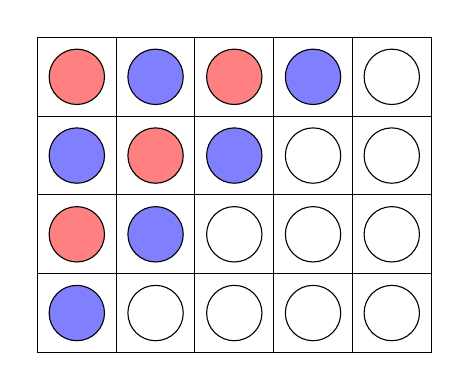
\begin{tikzpicture}[
    mycell/.style={draw, minimum size=1cm},
    dot1/.style={mycell,
        append after command={%
            \pgfextra \draw[fill=red!50, thin] (\tikzlastnode) 
                circle[radius=10pt]; \endpgfextra}},
    dot2/.style={mycell,
        append after command={%
            \pgfextra \draw[fill=blue!50, thin] (\tikzlastnode)  
                circle[radius=10pt]; \endpgfextra}}, 
    dot3/.style={mycell,
        append after command={%
            \pgfextra \draw[fill=white, thin] (\tikzlastnode)  
                circle[radius=10pt]; \endpgfextra}}, 
    ]

\matrix (m) [matrix of nodes, row sep=-\pgflinewidth, column sep=-\pgflinewidth, 
nodes={mycell}, nodes in empty cells]
{
  |[dot1]| & |[dot2]| & |[dot1]| & |[dot2]| & |[dot3]| \\
  |[dot2]| & |[dot1]| & |[dot2]| & |[dot3]| & |[dot3]| \\
  |[dot1]| & |[dot2]| & |[dot3]| & |[dot3]| & |[dot3]| \\
  |[dot2]| & |[dot3]| & |[dot3]| & |[dot3]| & |[dot3]| \\
};
\end{tikzpicture}

\end{document}
